\subsection{Reducibility of configurations on $R_5$}

Recall that every planar graph has a vertex with $\deg(v) \leq 5$. If we add edges between the neighbors of this vertex, then we obtain the rings $R_1$ thru $R_5$. We have seen the 0-reducibility of configurations on the first four. Therefore, if we could prove that every configuration on $R_5$ is 0-reducible, any planar graph would be reducible and the four color theorem would follow. Many people have tried to show this and failed, so let this serve as an warning as to why we should prove 1-reducibility instead.

\begin{theorem}
    A configuration $\confg$ on $R_5$ is 1-reducible in all planar graphs $M$ if it has a 3-coloring, or all planar graphs with $|M|>1$ if it does not.
\end{theorem}

\begin{proof}
We may consider a configuration with $|\confg| > 1$. Let the planar graph $M$ be arbitary. We will again use the convention of the sets $\I$ and $\II$ for the ring colorings.

\begin{equation}
    \I = \Phi(M+S) \quad \text{and} \quad \II = \Phi(\confg).
\end{equation}

The heart of this proof depends on a guaranteed 3-coloring in both $\I$ and $\II$. Because we may set our reducer $S=W_5$ (See Figure \ref{fig:reducertut}), we are guaranteed of the following colorings.
\begin{equation}
    \Phi^\star(5) \;\subset\; \I, \II \quad\text{and}\quad \Phi^{W_5} \subset \I,\II.
\end{equation}

To justify that $\Phi^{W_5} \subset \II$ in case a 3-coloring is not given by $\confg$ from the start, let us add a single vertex $v$ to the configuration $\confg$ as illustrated in Figure \ref{fig:confg3col}. This results in the graph $\confg'$ on 1 more vertex. We may assume that $\confg'$ has a 4-coloring because $\confg' < M+\confg$ from our assumption that $|M| > 1$. In particular, $\confg'$ will have a 3-coloring on the ring from $W_5$. We may remove $v$ in this 3-coloring to obtain a 3-coloring of $\confg$. Therefore $\Phi^{W_5} \subset \Phi(\confg)$. 

\needspace{5cm}
\begin{figure}
    \centering
    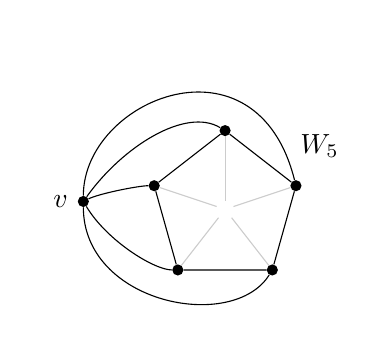
\begin{tikzpicture}
        \draw[opacity=0] (-0.5, 0) ellipse (2cm and 1.5cm);
        \node[fill=white] at (1.2, 0.8) {$W_5$};
        \node[inner sep=1mm] (c) at (0, 0) {$\core$};
        \node[circle, fill, scale=0.015cm] (l1) at (0, 1) { };
        \node[circle, fill, scale=0.015cm] (l2) at (0.9, 0.30) { };
        \node[circle, fill, scale=0.015cm] (l3) at (0.6, -0.77) {};
        \node[circle, fill, scale=0.015cm] (l4) at (-0.6, -0.77) {};
        \node[circle, fill, scale=0.015cm] (l5) at (-0.9, 0.30) {};
        \node[circle, fill, scale=0.015cm, label=left:$v$] (e) at (-1.8, 0.1) { };

        \draw (e) .. controls +(0.2, 0.1) and + (-0.2, 0.0) .. (l5);
        \draw (e) .. controls +(0.3, -0.5) and +(-0.3,0) .. (l4);
        \draw (e) .. controls +(0.0,-1.3) and +(-0.5,-0.8) .. (l3);
        \draw (e) .. controls +(0.0,+1.3) and +(-0.5,+2) .. (l2);
        \draw (e) .. controls +(0.5,0.7) and +(-0.5, 0.3) .. (l1);

        \draw[opacity=0.2] (c) -- (l1);
        \draw[opacity=0.2] (c) -- (l2);
        \draw[opacity=0.2] (c) -- (l3);
        \draw[opacity=0.2] (c) -- (l4);
        \draw[opacity=0.2] (c) -- (l5);
        \draw (l1) -- (l2) -- (l3) -- (l4) -- (l5) -- (l1);
    \end{tikzpicture}  
    \caption{The modified configuration $\confg'$ used to guarantee a 3-coloring of $\confg$.}
    \label{fig:confg3col}
\end{figure}


A special property of 3-colorings on $R_5$ is that there will always be a single vertex colored uniquely, we call this the \textit{marked vertex}. This vertex acts as a kind of 'pivot' to tell if two 3-colorings are \textit{adjacent}. These two concepts are key to the proof.

\begin{definition}
    The uniquely-colored vertex of a 3-coloring of $R_5$ is called the \emph{marked vertex}, indicated by an underline such as in $\underline{c}abab$.
\end{definition}
\begin{definition}
    Two 3-colorings of $R_5$ are called \emph{adjacent} if they have adjacent marked vertices, such as in $\underline{c}abab$ and $a\underline{c}bab$.
\end{definition}

Since we have guaranteed 3-colorings for both $\I$ and $\II$, we can split up our proof into 3 cases.

\begin{enumerate}
    \item $\I$ and $\II$ have an adjacent coloring ($\underline{c}abab$ and $a\underline{c}bab$).
    \item $\I$ and $\II$ have a non-adjacent coloring ($\underline{c}abab$ and $ab\underline{c}ab$).
    \item $\I$ and $\II$ have a coloring with the same marked vertex ($\underline{c}abab$ and $\underline{d}cbcb$). These are already equal, so we are done.
\end{enumerate}

Therefore, we only need to consider the cases \circled{1} and \circled{2}. We will prove two lemma's to this end. Their relation is illustrated below.

\begin{equation*}
    \begin{aligned}
    \circled{2} \implies\; &\circled{1}\quad \text{or} \quad \text{common coloring} \quad\quad \text{(Lemma \ref{lem:r5_first})} \\
    &\downarrow \\
    &\circled{1} \implies\;\text{common coloring}\quad\quad \text{(Lemma \ref{lem:r5_second})}
    \end{aligned}
\end{equation*}

\begin{lemma}
    \label{lem:r5_first}
    If $\I$ and $\II$ have a non-adjacent coloring, then they either have an adjacent coloring or a common coloring.
\end{lemma}

\begin{proof}
Let two non-adjacent colorings $\I(\underline{c}abab)$ and $\II(ab\underline{c}ab)$ be given. We make a case dinstinction whether the chain $v_3 \stackrel{bc}{\frown} v_5$ exists in $\II(ab\underline{c}ab)$ or not. 

\begin{equation}
    \label{eq:abcab}
    \begin{aligned}
        \II(ab\underline{c}ab) &=\scheme{a,b,c,a,b}{35b} \compat \II(abcdb), \\
        \II(ab\underline{c}ab) &= \scheme{a,b,c,a,b}{35b-} \compat \II(a\underline{c}bab).
    \end{aligned}
\end{equation}

The second case results in a coloring adjacent to $\I(\underline{c}abab)$. For the first case, we consider the coloring $\I({*}b{*}{*}b)$. The two adjacent ${*}$-colors must be different from each other and $b$, therefore we may assume that we have $\I({*}bcdb)$. The last ${*}$-color reveals 3 possibilities.

\begin{equation}
    \begin{matrix*}[l]
        \I(abcdb) \quad\quad =&\II(abcdb) \; \text{from (\ref{eq:abcab}),}  \\
        \I(cbc\underline{d}b) \;\; \text{adjacent to}&\II(ab\underline{c}ab), \;  \\
        \I(db\underline{c}db) \quad\quad =&\II(ab\underline{c}ab).
    \end{matrix*}
\end{equation}

Therefore we obtain either a common coloring or an adjacent coloring. Note that the pair of non-adjacent colorings we chose is the only unique one on $R_5$ (up to rotational symmetry).
\end{proof}

\begin{lemma}
    \label{lem:r5_second}
    If I and II have an adjacent coloring, then they have a common coloring.
\end{lemma}

\begin{proof}

Let two adjacent colorings $\I(\underline{c}abab)$ and $\II(a\underline{c}bab)$ be given. We make a case dinstinction whether the chain $\chain{v_3}{v_5}{bd}$ exists in $\II(a\underline{c}bab)$ or not.

\begin{equation}
    \label{eq:acdab}
    \begin{aligned}
        \II(a\underline{c}bab) &= \scheme{a,c,b,a,b}{35d} \compat \I(\underline{c}abab). \\
        \II(a\underline{c}bab) &= \scheme{a,c,b,a,b}{35d-} \compat \II(acdab).
    \end{aligned}
\end{equation}

The first case leads to a common coloring. For the second case,
we consider the coloring $\I(a{*}{*}a{*})$. We may again assume to have $\I(acda{*})$. Then the 3 remaining possibilities for the ${*}$-color are

\begin{equation*}
    \begin{matrix*}[l]
        \I(acdab) \quad =& \II(acdab), \;\text{from (\ref{eq:acdab})},\\
        \I(ac\underline{d}ac) \quad =\;\; \text{shifted $+2$}& \I(\underline{c}abab), \\
        \I(a\underline{c}dad) \quad =& \II(a\underline{c}bab).
    \end{matrix*}
\end{equation*}

If we do not obtain common colorings, we may repeat this procedure with $\II(a\underline{c}bab)$ and $\I(ac\underline{d}ac)$ to continously shift the marked vertex two to the right. The pattern that arises is illustrated in Figure \ref{table:ringpattern5}.

\begin{figure}[!ht]
    \centering
    \begin{tabular}{c|ccccc:c}
         & $v_1$ & $v_2$  & $v_3$  & $v_4$ & $v_5$ & $v_1$  \\
        \hline
        1 & \I & \II &    &     &    & \I  \\
        2 &    & \II & \I &     &    &     \\
        3 &    &     & \I & \II &    &     \\
        4 &    &     &    & \II & \I &     \\
        5 &    &     &    &     & \I & \II \\
    \end{tabular}
    \caption{Marked vertices of $\I$ and $\II$ obtained by repetition of the earlier procedure.  Every step shifts the leftmost marked vertex two to the right. }
    \label{table:ringpattern5}
\end{figure}

At iteration 5, we obtain that $\II$ has the same marked vertex $v_1$ as $\I$. Therefore, by repetition we obtain that

\begin{equation}
    \II(a\underline{c}bab) \rightarrow \II(aba\underline{c}b) \rightarrow \II(\underline{c}abab) = \I(\underline{c}abab).
\end{equation}

\end{proof}

Therefore, adjacent colorings imply a common coloring for $\I$ and $\II$. Combining these two lemmas yields a guaranteed common ring coloring for $\I$ and $\II$ regardless of the case.

\end{proof}